%  Example for the ETH Beamer template
%  Copyright 2014 by 
%  Dr. Antonios Garas,
%  Chair of Systems Design, ETH Zurich
%  Weinbergstrasse 56/58 CH-8092 Zurich
%
%To compile this into a pdf, install the latex-beamer package which provides the latex-beamer.cls
\documentclass[
%aspectratio=169,
first,
%handout,
%compress,
%Helv,
ETH1,
navigation
]{ETHbeamerclass} 

% Options for beamer:
% 
% compress: navigation bar becomes smaller
% t       : place contents of frames on top (alternative: b,c)
% handout : handoutversion
% notes   : show notes
% notes=onlyslideswithnotes
%
\setbeamertemplate{note page}{\ \\[.3cm]
\textbf{\color{colorSG}Notes:}\\%[0.1cm]
{\footnotesize %\tiny
\insertnote}}

\setbeameroption{hide notes}
%\setbeameroption{show notes}

\setbeamertemplate{navigation symbols}{} % suppresses all navigation symbols:
% \setbeamertemplate{navigation symbols}[horizontal] % Organizes the navigation symbols horizontally.
% \setbeamertemplate{navigation symbols}[vertical] % Organizes the navigation symbols vertically.
% \setbeamertemplate{navigation symbols}[only frame symbol] % Shows only the navigational symbol for navigating frames.

\usepackage{amsmath, amssymb}
%\usepackage{tikz, tkz-graph}
\usepackage{pifont}
%\usepackage{subfig}
%\usepackage{natbib}
\usepackage{tikz}
\usetikzlibrary{decorations.pathreplacing}
\usepackage{multimedia}

%--------------------------------------------------------------------------------------------------------
%--- Some custom definitions...

\definecolor{cbf}{RGB}{199,100,95}%{163,15,0}
\newcommand{\cbf}{\color{cbf}}

\newcommand{\mean}[1]{\left\langle #1 \right\rangle}
\newcommand{\abs}[1]{\left| #1 \right|}

%--------------------------------------------------------------------------------------------------------
%--- Inputs for the title page...

\title{On the origin of creatures\\
The evolution of virtual creatures in a
rigid-body engine
}
\newcommand{\shorttitle}{Shorter title}

\author{Benjamin Ellenberger}
\date{\today}
\institute{INI:  Institute of Neuroinformatics}

\newcommand{\collaborators}{}
\newcommand{\event}{Neuronal networks}
\newcommand{\place}{}

\newcommand{\Prob}{\mathrm{Pr}}
\newcommand{\sign}{\mathrm{sign}}
\newcommand{\R}{\mathbb{R}}
\newcommand{\N}{\mathbb{N}}
\newcommand{\nbin}[1]{\mathrm{nb}_\mathrm{in}(#1)}
\newcommand{\nbout}[1]{\mathrm{nb}_\mathrm{out}(#1)}
\newcommand{\one}{\mathbb{\bf 1}}

\newcommand{\sref}[1]{SLIDE \ref{#1}}

%--------------------------------------------------------------------------------------------------------
%--- Here begins the presentation...

\begin{document}

\frame{
\maketitle
}
\note{}


\section{Introduction}

\frame{

  \frametitle{Contents}
    \tableofcontents[currentsection]
}
\note{}

\subsection{Karl Sims}
\frame{

  \frametitle{Karl Sims}
  
    \begin{columns}
   \column{0.6\textwidth}
  \begin{itemize}
    \item Computer artist and researcher from MIT Media Lab in the 1990s
      \item Wrote landmark papers on virtual creatures and artificial evolution
     \end{itemize}
      

  \column{0.35\textwidth}
  \includegraphics[height=2.15in, clip] {figs/Karl-Sims-l.jpg}   
  \end{columns}

      \begin{itemize}
    \item Panspermia, 1990, Animation depicting a life cycle of an inter-galactic botanical life form. 
      \item Evolved Virtual Creatures, 1994, Demonstration of research results show simulated block creatures performing various evolved behaviors.
     \end{itemize}
  }
\note{}

\frame{

  \frametitle{Evolved Virtual Creatures}
  
  \begin{columns}
   \column{0.6\textwidth}
 \begin{itemize}
	     \item Simulations were created on the IBM CM-5 (1024 cores, 32 GFlops/s) 
    	\item The creatures were evolved to display multiple modes of water and land based movements 
    	\item The creatures were also co-evolved in different species to compete for possession of a virtual cube, displaying the red queen effect. 
     \end{itemize}
     
     \column{0.35\textwidth}
      \includegraphics[height=1in, clip] {figs/CM5.jpg}\\
      \includegraphics[width=1.5in, clip] {figs/creatures.jpg} 
  \end{columns}
  }
\note{}


\section{Methods}

\frame{

  \frametitle{Contents}
    \tableofcontents[currentsection]
}
\note{}

\subsection{Genetic language}
\frame{

  \frametitle{Genetic language}
  
Genotype:
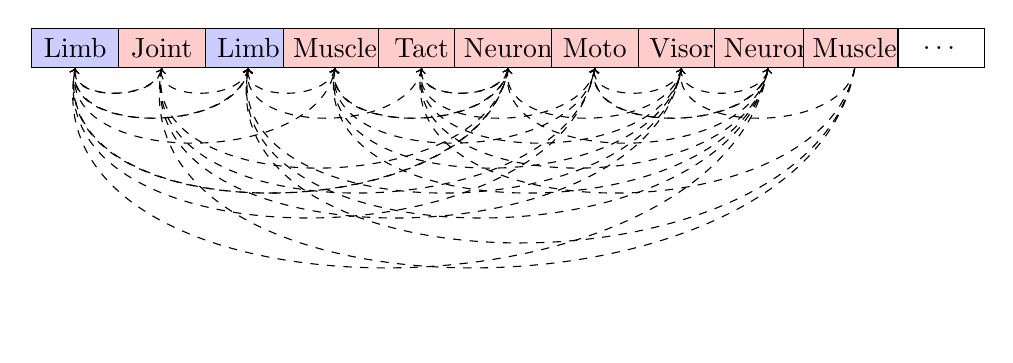
\begin{tikzpicture}
   \foreach \c/\i [count=\n] in  
        {blue!20/Limb,red!20/Joint,blue!20/Limb,red!20/Muscle,red!20/Tact,red!20/Neuron,red!20/Moto,red!20/Visor,red!20/Neuron,red!20/Muscle,white/\dots} 
           \node[draw,fill=\c,minimum height=0.5cm,minimum width = 1.1cm,xshift=\n*1.1cm](N\n){\i} ;
\draw[dashed,->] (N1.south) to [out=-100,in=-100] (N2.south);
\draw[dashed,->] (N1.south) to [out=-100,in=-100] (N3.south);
\draw[dashed,->] (N1.south) to [out=-100,in=-100] (N4.south);
\draw[dashed,->] (N1.south) to [out=-100,in=-100] (N6.south);

\draw[dashed,->] (N2.south) to [out=-100,in=-100] (N7.south);
\draw[dashed,->] (N2.south) to [out=-100,in=-100] (N6.south);
\draw[dashed,->] (N2.south) to [out=-100,in=-100] (N8.south);
\draw[dashed,->] (N2.south) to [out=-100,in=-100] (N1.south);

\draw[dashed,->] (N3.south) to [out=-100,in=-100] (N8.south);
\draw[dashed,->] (N3.south) to [out=-100,in=-100] (N3.south);
\draw[dashed,->] (N3.south) to [out=-100,in=-100] (N2.south);
\draw[dashed,->] (N3.south) to [out=-100,in=-100] (N1.south);

\draw[dashed,->] (N4.south) to [out=-100,in=-100] (N6.south);
\draw[dashed,->] (N4.south) to [out=-100,in=-100] (N7.south);
\draw[dashed,->] (N4.south) to [out=-100,in=-100] (N4.south);
\draw[dashed,->] (N4.south) to [out=-100,in=-100] (N3.south);

\draw[dashed,->] (N5.south) to [out=-100,in=-100] (N3.south);
\draw[dashed,->] (N5.south) to [out=-100,in=-100] (N6.south);
\draw[dashed,->] (N5.south) to [out=-100,in=-100] (N8.south);
\draw[dashed,->] (N5.south) to [out=-100,in=-100] (N9.south);

\draw[dashed,->] (N6.south) to [out=-100,in=-100] (N5.south);
\draw[dashed,->] (N6.south) to [out=-100,in=-100] (N4.south);
\draw[dashed,->] (N6.south) to [out=-100,in=-100] (N1.south);
\draw[dashed,->] (N6.south) to [out=-100,in=-100] (N9.south);

\draw[dashed,->] (N7.south) to [out=-100,in=-100] (N1.south);
\draw[dashed,->] (N7.south) to [out=-100,in=-100] (N7.south);
\draw[dashed,->] (N7.south) to [out=-100,in=-100] (N5.south);
\draw[dashed,->] (N7.south) to [out=-100,in=-100] (N9.south);

\draw[dashed,->] (N8.south) to [out=-100,in=-100] (N9.south);
\draw[dashed,->] (N8.south) to [out=-100,in=-100] (N4.south);
\draw[dashed,->] (N8.south) to [out=-100,in=-100] (N6.south);
\draw[dashed,->] (N8.south) to [out=-100,in=-100] (N7.south);

\draw[dashed,->] (N9.south) to [out=-100,in=-100] (N4.south);
\draw[dashed,->] (N9.south) to [out=-100,in=-100] (N7.south);
\draw[dashed,->] (N9.south) to [out=-100,in=-100] (N1.south);
\draw[dashed,->] (N9.south) to [out=-100,in=-100] (N3.south);

\draw[dashed,->] (N10.south) to [out=-100,in=-100] (N2.south);
\draw[dashed,->] (N10.south) to [out=-100,in=-100] (N8.south);
\draw[dashed,->] (N10.south) to [out=-100,in=-100] (N5.south);
\draw[dashed,->] (N10.south) to [out=-100,in=-100] (N3.south);
\end{tikzpicture}

\begin{columns}
   \column{0.45\textwidth}
  \begin{itemize}
\item \textbf{Limb} Part of creature body
\item \textbf{Joint} Generic joint
\item \textbf{Muscle} Muscle of Joint
\end{itemize}

  \column{0.45\textwidth}
    \begin{itemize}
    \item \textbf{Tact} Tactile Sensor
\item \textbf{Moto} Motorceptor (Force)
\item \textbf{Visor} Light sensor
\end{itemize}
  \end{columns}
  
  }
\note{}

\frame{
 \frametitle{Genetic language}
Phenotype:
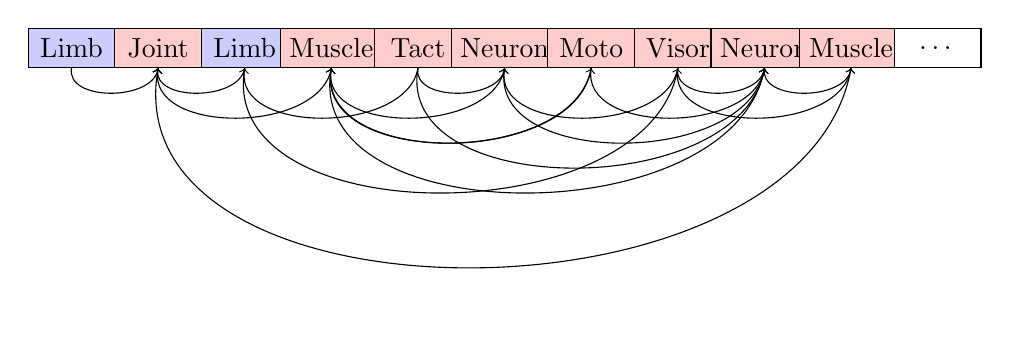
\begin{tikzpicture}
  
  
   \foreach \c/\i [count=\n] in  
        {blue!20/Limb,red!20/Joint,blue!20/Limb,red!20/Muscle,red!20/Tact,red!20/Neuron,red!20/Moto,red!20/Visor,red!20/Neuron,red!20/Muscle,white/\dots} 
           \node[draw,fill=\c,minimum height=0.5cm,minimum width = 1.1cm,xshift=\n*1.1cm](N\n){\i} ;
\draw[->] (N1.south) to [out=-100,in=-100] (N2.south);



\draw[->] (N3.south) to [out=-100,in=-100] (N8.south);
\draw[->] (N3.south) to [out=-100,in=-100] (N2.south);

\draw[->] (N4.south) to [out=-100,in=-100] (N7.south);
\draw[->] (N4.south) to [out=-100,in=-100] (N2.south);

\draw[->] (N5.south) to [out=-100,in=-100] (N3.south);
\draw[->] (N5.south) to [out=-100,in=-100] (N6.south);
\draw[->] (N5.south) to [out=-100,in=-100] (N9.south);

\draw[->] (N6.south) to [out=-100,in=-100] (N4.south);
\draw[->] (N6.south) to [out=-100,in=-100] (N9.south);

\draw[->] (N7.south) to [out=-100,in=-100] (N4.south);
\draw[->] (N7.south) to [out=-100,in=-100] (N9.south);

\draw[->] (N8.south) to [out=-100,in=-100] (N9.south);
\draw[->] (N8.south) to [out=-100,in=-100] (N10.south);
\draw[->] (N8.south) to [out=-100,in=-100] (N6.south);

\draw[->] (N9.south) to [out=-100,in=-100] (N4.south);
\draw[->] (N9.south) to [out=-100,in=-100] (N10.south);


\draw[->] (N10.south) to [out=-100,in=-100] (N2.south);
\end{tikzpicture}

\begin{columns}
   \column{0.45\textwidth}
  \begin{itemize}
\item \textbf{Limb} Part of creature body
\item \textbf{Joint} Generic joint
\item \textbf{Muscle} Muscle of Joint
\end{itemize}

  \column{0.45\textwidth}
    \begin{itemize}
    \item \textbf{Tact} Tactile Sensor
\item \textbf{Moto} Motorceptor (Force)
\item \textbf{Visor} Light sensor
\end{itemize}
  \end{columns}
  }
\note{}


\subsection{Neuronal network}
\frame{

  \frametitle{Neuronal network}
  


\begin{columns}
   \column{0.55\textwidth}
  Each neuron has a transfer function, which is one of: 

\begin{columns}
   \column{0.45\textwidth}
   \begin{itemize}
    \item min
\item max
\item sum
\item sum-theshold
\item product
\item abs
    \item sign-of
\end{itemize}
   \column{0.45\textwidth}
   \begin{itemize}

\item greater-than
\item exp
\item log
\item sin
\item cos
\item oscillate-wave
\item oscillate-saw
\end{itemize}
  \end{columns}
  \column{0.35\textwidth}
\includegraphics[width=1.5in, clip] {figs/NN.png} 
  \end{columns}

  
  }
\note{}

\subsection{Oja's rule}
\frame{

  \frametitle{Oja's rule}
  
  \begin{columns}
   \column{0.45\textwidth}
   \begin{itemize}
   \item Finnish computer scientist Erkki Oja
   \item $x$ is the input
   \item $y(x)$ is the output
   \item $w_i(n+1)$ is the new weight
   \item For $p = 2$, we have the root sum of squares\\ (Cartesian normalization rule)
   \item Stabilized rule of Hebb's learning rule $\Delta w_i = \eta x_i y $
   \end{itemize}
      \column{0.45\textwidth}
  \begin{align*}
w_i (n+1) ~ = ~ \frac{w_i + \eta\, y(\mathbf{x}) x_i}{\left(\sum_{j=1}^m [w_j + \eta\, y(\mathbf{x}) x_j]^p \right)^{1/p}}
\end{align*}
\end{columns}
  
  }
\note{}

\subsection{Hill's muscle model}
\frame{

  \frametitle{Hill's muscle model}
  
    \begin{columns}
   \column{0.6\textwidth}
    \begin{itemize}
    \item Physiologist Archibald Vivian Hill
    \item Equation of tetanized muscle contraction
  \item $\left(v+b\right)(F+a) = b(F_0+a)$
  \begin{itemize}
  \item $F$ is the tension (or load) in the muscle
\item $v$ is the velocity of contraction
\item $F_0$ is the maximum isometric tension\\ (or load) generated in the muscle
\item a coefficient of shortening heat
\item $b=a\cdot v_0/F_0$
\item $v_0$ is the maximum velocity, when $F=0$
  \end{itemize}
  \end{itemize}
      \column{0.3\textwidth}
      \includegraphics[width=1.5in, clip] {figs/Hill-model.png}
  \end{columns}

  
  }
\note{}

\frame{

  \frametitle{Execution of creatures}
\includegraphics[width=2.3in, clip] {figs/brain-body-cycle.png}
\includegraphics[width=2.5in, clip] {figs/execution.png}
  
  }
\note{}

\subsection{Fitness evaluation}
\frame{

  \frametitle{Fitness evaluation}

\begin{itemize}
\item Fitness evaluation framework
\item A creature is simulated for a certain evaluation time during which the fitness function measures the fitness of the creature
\item Evaluates multiple fitness functions at the same time and combines them linearly
\end{itemize}

  
  }
\note{}

\subsection{Evolution}
\frame{

  \frametitle{Evolution}

\begin{itemize}
\item Selection
\begin{itemize}
\item Only a certain percentage of creatures are selected for new generation
\end{itemize}
\item Cross-over
\begin{itemize}
\item Only certain percentage of creatures are allowed to breed
\end{itemize}
\item Mutation
\begin{itemize}
\item Other creatures are subject to mutation
\item Mutation of gene
\item Mutation of gene attributes
\item Mutation of gene links
\end{itemize}
\item Successful creatures stay in the population and the population is refilled with new bred and mutated ones
\end{itemize}
  
  }
\note{}



\section{Simulations}

\frame{

  \frametitle{Contents}
    \tableofcontents[currentsection]
}
\note{}

\subsection{Velocity as the fitness function}
\frame{

  \frametitle{Velocity as the fitness function}

\begin{itemize}
\item Sampling of position over time
\item Moved distance in a certain time interval
\item Continuous average
\item Expectations: Some really moving creatures and some finding the exploit that only the main body has to move. \\(main body = first limb in phenotype)
\end{itemize}
  
  }
\note{}

\subsection{First run}
\frame{

  \frametitle{First run}
      \begin{columns}
   \column{0.25\textwidth}
   \begin{itemize}
   \item 20 Individuals
   \item 30 generations
   \item Check if they can exploit the fitness function
   \item Result: There was another exploit in the virtual world!
   \end{itemize}
    \column{0.6\textwidth}
\includegraphics[width=3in, clip] {figs/velocity1.png}
\end{columns}
  
  }
\note{}

\subsection{Second run}
\frame{

  \frametitle{Second run}
        \begin{columns}
   \column{0.25\textwidth}
      \begin{itemize}
   \item 20 Individuals
   \item 30 generations
   \item The problem of the previous run is fixed
   \item Check if they can exploit the fitness function
   \item Result: They found several exploitation strategies!
   \end{itemize}
       \column{0.6\textwidth}
\includegraphics[width=3in, clip] {figs/velocity2.png}
\end{columns}
  
  }
\note{}

\frame{

  \frametitle{Creatures}
  \begin{figure}[tp]
    \centering
    \includegraphics[width=3in, clip] {figs/c2.png}
\end{figure}
  }
\note{}

\frame{

  \frametitle{Creatures}
  \begin{figure}[tp]
    \centering
    \includegraphics[width=3in, clip] {figs/c3.png}
\end{figure}
  }
\note{}

\frame{

  \frametitle{Creatures}
  \begin{figure}[tp]
    \centering
    \includegraphics[width=3in, clip] {figs/c5.png}
\end{figure}
  }
\note{}

\frame{

  \frametitle{Creatures}
  \begin{figure}[tp]
    \centering
    \includegraphics[width=3in, clip] {figs/c6.png}
\end{figure}
  }
\note{}

\frame{

  \frametitle{Creatures}
  \begin{figure}[tp]
    \centering
    \includegraphics[width=3in, clip] {figs/c7.png}
\end{figure}
  }
\note{}

\frame{

  \frametitle{Creatures}
  \begin{figure}[tp]
    \centering
    \includegraphics[width=3in, clip] {figs/c8.png}
\end{figure}
  }
\note{}

\frame{

  \frametitle{Creatures}
  \begin{figure}[tp]
    \centering
    \includegraphics[width=3in, clip] {figs/c9.png}
\end{figure}
  }
\note{}

\frame{

  \frametitle{Creatures}
  \begin{figure}[tp]
    \centering
    \includegraphics[width=3in, clip] {figs/c10.png}
\end{figure}
  }
\note{}

\frame{

  \frametitle{Creatures}
  \begin{figure}[tp]
    \centering
    \includegraphics[width=3in, clip] {figs/c11.png}
\end{figure}
  }
\note{}

\frame{

  \frametitle{Creatures}
  \begin{figure}[tp]
    \centering
    \includegraphics[width=3in, clip] {figs/c12.png}
\end{figure}
  }
\note{}

\frame{

  \frametitle{Creatures}
  \begin{figure}[tp]
    \centering
    \includegraphics[width=3in, clip] {figs/c13.png}
\end{figure}
  }
\note{}

\frame{

  \frametitle{Creatures}
  \begin{figure}[tp]
    \centering
    \includegraphics[width=3in, clip] {figs/c14.png}
\end{figure}
  }
\note{}

\frame{

  \frametitle{Creatures}
  \begin{figure}[tp]
    \centering
    \includegraphics[width=3in, clip] {figs/c15.png}
\end{figure}
  }
\note{}

\frame{

  \frametitle{Creatures}
  \begin{figure}[tp]
    \centering
    \includegraphics[width=3in, clip] {figs/c16.png}
\end{figure}
  }
\note{}


\section{Outlook}

\frame{

  \frametitle{Contents}
    \tableofcontents[currentsection]
}
\note{}

\subsection{Optimization \& Extension}
\frame{

  \frametitle{Optimization \& Extension}
  
  \begin{itemize}
  \item The framework was written in a quick \& dirty manner
  \item Several components need to be reimplemented properly to provide a more scalable environment
  \item The system does not use any parallelization
  \item The phenotype could be more natural
  \item The genotype to phenotype transcription does not include any additional developmental parts (no embryogenesis)
  \item More sensor types
  \item More logging for data analysis
  \end{itemize}
}
\note{}
\subsection{Other settings \& fitness functions}
\frame{

  \frametitle{Other settings \& fitness functions}
  \begin{itemize}
  \item Island genetic algorithm
  \item Competitions of individuals
  \item Implicit fitness functions (survival of the fittest in a virtual world)
  \item Information theoretic measures such as the transfer entropy
  \end{itemize}
}
\note{}


\frame{

  \frametitle{References}
  \begin{itemize}
  \item Sims K. - Evolving Virtual Creatures (1994)
  \item Sims K. - Evolving 3D Morphology and Behavior by Competition (1994)
  \item Krcah P. - Evolving Virtual Creatures Revisited (2007)
  \item Schmidt N. - Bootstrapping perception using information theory: case studies in a quadruped running robot running on different grounds (2013)
  \item Hill, A.V. The heat of shortening and dynamics constants of muscles  (1938)
  \item Stoop R. - Theory and Simulation of Neural Networks (2014)
  \end{itemize}
}
\note{}
\end{document}
